\documentclass[12pt, a4paper]{article}

% Required Packages
\usepackage{amsmath, graphicx}
\usepackage{amssymb}
\usepackage{kotex} % For Korean text
\usepackage{geometry}
\geometry{a4paper, margin=1in}
\graphicspath{{graph/}}
% Title
\title{Calculus - Chapter 9 Review Selected Exercises}
\author{}
\date{}

\begin{document}
\maketitle
\hrulefill
\vspace{1em}

\section*{Concept Check}
\begin{enumerate}
    \item (a) What is a differential equation? \\
          (b) What is the order of a differential equation? \\
          (c) What is an initial condition?

    \item What can you say about the solutions of the equation $y' = x^2 + y^2$ just by looking at the differential equation?

    \item What is a direction field for the differential equation $y' = F(x,y)$?

    \item Explain how Euler's method works.

    \item What is a separable differential equation? How do you solve it?
\end{enumerate}

\hrulefill
\vspace{1em}

\section*{True-False Quiz}
\begin{enumerate}
    \item All solutions of the differential equation $y' = -1 - y^4$ are decreasing functions.

    \item The function $f(x) = (\ln x)/x$ is a solution of the differential equation $x^2y' + xy = 1$.

    \item The function $y = 3e^{2x} - 1$ is a solution of the initial-value problem $y' - 2y = 1, y(0)=2$.

    \item The equation $y' = x+y$ is separable.
    
    \item The equation $y' = 3y - 2x + 6xy - 1$ is separable.
\end{enumerate}

\hrulefill
\vspace{1em}
\\
\section*{Exercises}
\begin{enumerate}
    \item (a) A direction field for the differential equation $y' = y(y-2)(y-4)$ is shown. Sketch the graphs of the solutions that satisfy the given initial conditions. \\
    (i) $y(0) = -0.3$ \quad (ii) $y(0) = 1$ \quad (iii) $y(0) = 3$ \quad (iv) $y(0) = 4.3$ \\
    (b) If the initial condition is $y(0)=c$, for what values of c is $\lim_{t \to \infty} y(t)$ finite? What are the equilibrium solutions?
     \begin{figure}[htbp] % [h!] 옵션은 여기에(here!) 그림을 위치시키라는 의미
        \centering % 이미지를 가운데로 정렬
       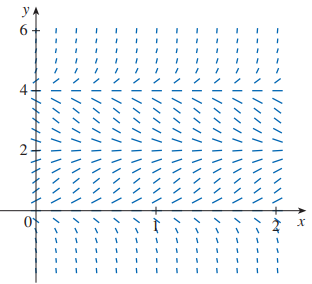
\includegraphics[width=0.4\textwidth]{graph5.png} % 너비는 텍스트 너비의 70%    
   \end{figure}

    \item (a) Sketch a direction field for the differential equation $y' = x/y$. Then use it to sketch the four solutions that satisfy the initial conditions $y(0)=1, y(0)=-1, y(2)=1,$ and $y(-2)=1$. \\
    (b) Check your work in part (a) by solving the differential equation explicitly. What type of curve is each solution curve?
    
    \item (a) A direction field for the differential equation $y' = x^2 - y^2$ is shown. Sketch the solution of the initial-value problem $y' = x^2 - y^2, y(0)=1$. \\
    \begin{figure}[htbp] % [h!] 옵션은 여기에(here!) 그림을 위치시키라는 의미
        \centering % 이미지를 가운데로 정렬
       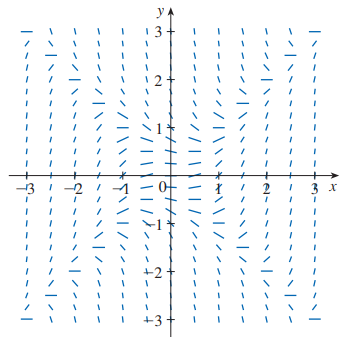
\includegraphics[width=0.4\textwidth]{graph6.png} % 너비는 텍스트 너비의 70%    
   \end{figure}
    (b) Use Euler's method with step size 0.1 to estimate $y(0.3)$.\\
    (c) On what lines are the centers of the horizontal line segments of the direction field in part (a) located? What happens when a solution curve crosses these lines?

    \item (a) Use Euler's method with step size 0.2 to estimate $y(0.4)$, where $y(x)$ is the solution of the initial-value problem $y' = 2xy^2, y(0)=1$. \\
    (b) Repeat part (a) with step size 0.1.\\
    (c) Find the exact solution of the differential equation and compare the value at 0.4 with the approximations in parts (a) and (b).
    
    \setcounter{enumi}{5} % Jumps to question 6
    \item Solve the differential equation.
    \[ \frac{dx}{dt} = 1 - t + x - tx \]
    
    \item Solve the differential equation.
    \[ 2ye^{y^2}y' = 2x + 3\sqrt{x} \]
    
    \setcounter{enumi}{8} % Jumps to question 9
    \item Solve the initial-value problem.
    \[ \frac{dr}{dt} + 2tr = r, \quad r(0)=5 \]
    
    \item Solve the initial-value problem.
    \[ (1+\cos x)y' = (1+e^{-y})\sin x, \quad y(0)=0 \]
    
    \setcounter{enumi}{11} % Jumps to question 12
    \item Solve the initial-value problem $y' = 3x^2e^y, y(0)=1$ and graph the solution.
    
    \item Find the orthogonal trajectories of the family of curves.
    \[ y = ke^x \]
    
    \item Find the orthogonal trajectories of the family of curves.
    \[ y = e^{kx} \]
    
    \item (a) Write the solution of the initial-value problem $\frac{dP}{dt} = 0.1P(1 - \frac{P}{2000}), P(0)=100$. \\
    (b) When does the population reach 1200?
    
    \setcounter{enumi}{17} % Jumps to question 18
    \item A tank contains 100 L of pure water. Brine that contains 0.1 kg of salt per liter enters the tank at a rate of 10 L/min. The solution is kept thoroughly mixed and drains from the tank at the same rate. How much salt is in the tank after 6 minutes?

\end{enumerate}

\end{document}
